\documentclass{ltjsarticle}
\usepackage{amsmath}
\usepackage{amssymb}
\usepackage{ascmac}
\usepackage[dvipdfmx]{graphicx}
\usepackage{tabularx}
\usepackage[colorlinks=true, allcolors=blue]{hyperref}
\usepackage{fancybox}
\usepackage{tikz}
\usepackage{subcaption}
\usetikzlibrary{shapes,arrows}

\begin{document}

\title{400. 深層学習の説明性}
\author{秋葉洋哉}
\maketitle

\section{解釈性の重要さ}
\subsection{概要}
ディープラーニング活用の難しいことの一つは「ブラックボックス性」にあるといえる。つまり、モデルの出力の根拠を説明することができないということである。
例えば、医療現場においては、患者の診断結果を説明できないモデルを用いることは困難である。そのため、モデルの解釈性を高めることが求められている。
\par
ディープラーニングモデルの解釈に使われる四つの手法として、
\begin{itemize}
  \item CAM
  \item Grad-CAM
  \item LIME
  \item SHAP
\end{itemize}
がある。以下では、それぞれの手法について説明する。

\subsection{CAM}
CAM(Class Activation Map)は、正則化の役割のあったGlobal Average Poolingを再検討し、CNNが潜在的に注目している部分を可視化できるようにする役割を持っていることが明らかになったことで、提案された手法である。直観的には、出力層の重みを畳み込み特徴マップに投影することで、画像領域の重要性を識別することができる(図\ref{fig:CAM})。
ただし、CAMが利用できるネットワークは、CNNを大部分で使用しており、出力層前にGAPを実行していることが前提となる。
\begin{figure}
  \centering
  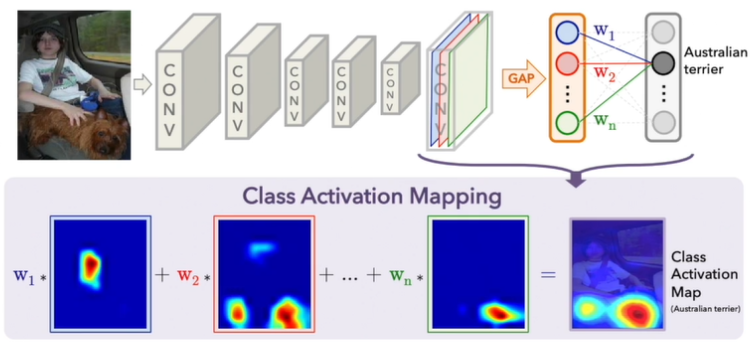
\includegraphics[width=13cm]{./capture/CAM.png}
  \caption{GAP後の各セルの重みと、GAP直前のCNN層のフィルタの重みを掛け合わせることで、Class Activation Mapが出力される。}
  \label{fig:CAM}
\end{figure}
数式で表すと、
\begin{align}
  M_c(x,y) = \sum_{k} w_k^c f_k(x,y)
\end{align}
で表される。
CAMを用いてモデルがどこに注目しているかを可視化した図を、図\ref{fig:CAM_example}に示す。
\begin{figure}[htbp]
  \centering
  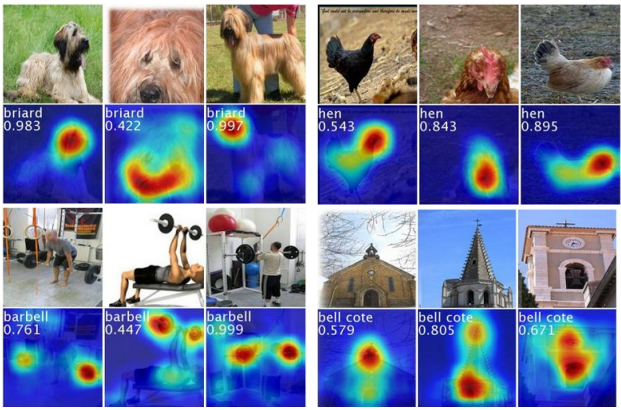
\includegraphics[width=13cm]{./capture/CAM_example.png}
  \caption{CAMを用いてモデルがどこに注目しているかを可視化した図}
  \label{fig:CAM_example}
\end{figure}

\subsection{Grad-CAM}
Grad-CAMとは、CAMと同様、CNNモデルに判断根拠を持たせ、モデルの予測根拠を可視化する手法である。Grad-CAMは、CAMでのGAPの代わりに、最後のCNN層の勾配を用いて、特徴マップを抽出する。この性質から、最後にGAPを用いないネットワークにも適用することができる。勾配が大きいピクセルほど、モデルが注目していると考えられる。
\par
また、Grad-CAMは、CAMと比較して、ネットワークの構造に依存しないため、画像分類だけでなく、物体検知やセグメンテーションにも適用できる。
\par
Grad-CAMのヒートマップがどのように生成されるかを示した図を、図\ref{fig:Grad-CAM}に示す。
\begin{figure}
  \centering
  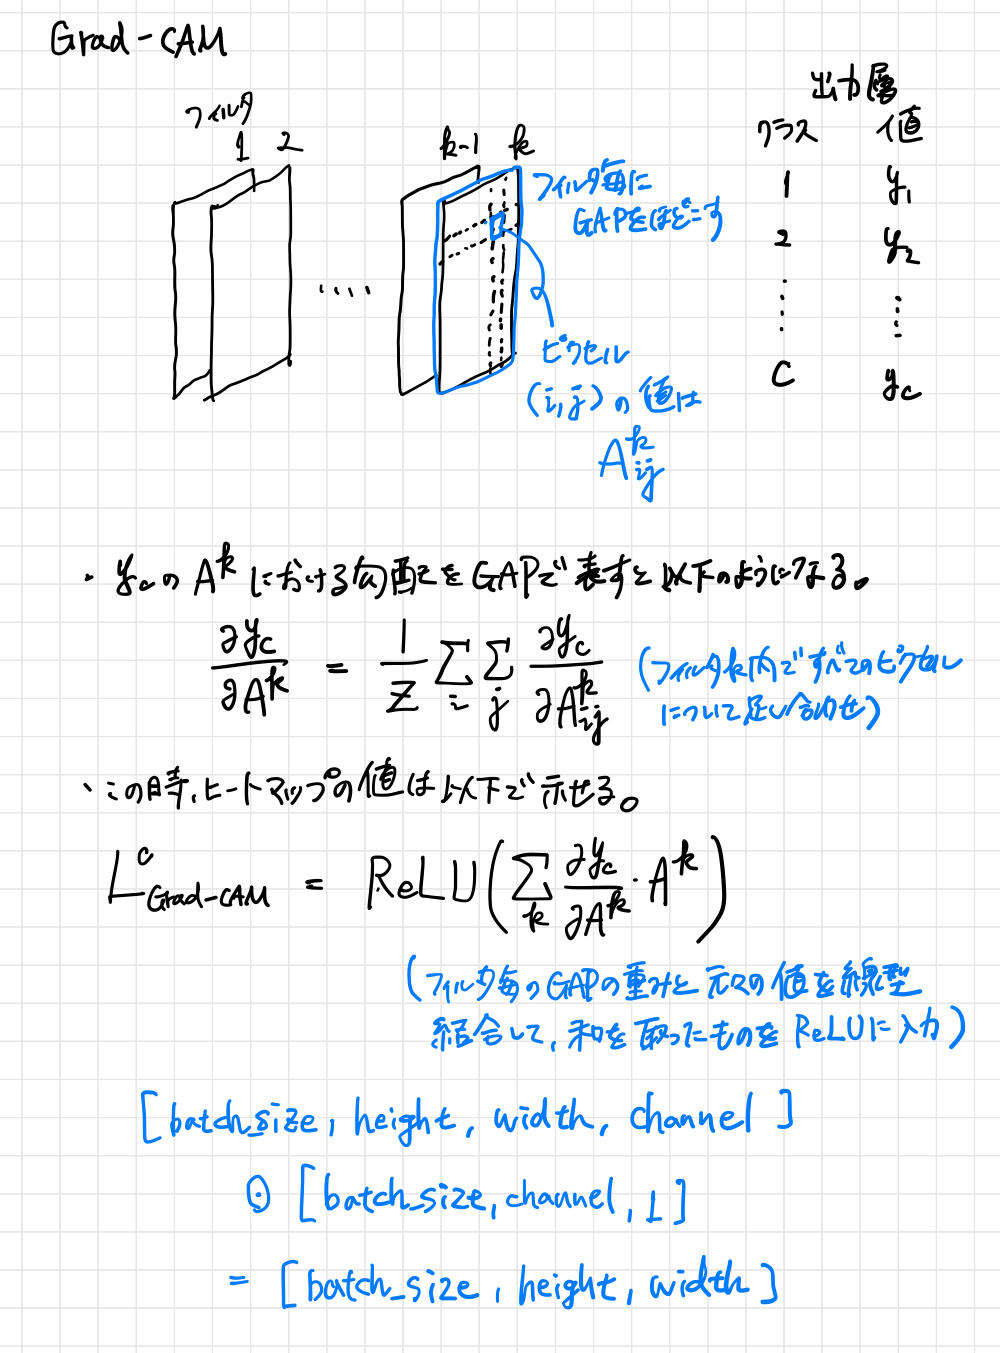
\includegraphics[width=14cm]{./capture/Grad-CAM.png}
  \caption{Grad-CAMのヒートマップ生成過程}
  \label{fig:Grad-CAM}
\end{figure}

\clearpage
\section{LIME}
LIME(Local Interpretable Model-agnostic Explanations)は、特定の入力データに対する予測について、その判断根拠を解釈・可視化するツールのことを指す。例えば、表形式データを入力したとき、どの変数が予測に寄与しているか、また、画像データを入力したとき、どのピクセルが予測に寄与しているかを可視化することができる。
\par
LIMEは、複雑なモデルをシンプルなモデル(決定木等)で線形近似し、その近似モデルを解釈することで、モデルの予測根拠を解釈する。LIMEの手法は、以下の手順で行われる。
\par
\begin{enumerate}
  \item 入力:一つの個別の予測結果
  \item 近似モデル:入力データに類似したデータ(領域削除・反転・ランダム置換等)をサンプリングし、そのデータを教師データとして、データ空間の対象範囲内でのみ有効な線形近似モデルを作成
  \item 出力:近所用モデルから予測に寄与した特徴量を選び解釈を行うことで、本来の難解なモデルの予測根拠を解釈(したとみなす)
\end{enumerate}

\begin{figure}[htbp]
  \centering
  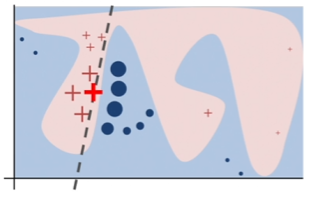
\includegraphics[width=14cm]{./capture/LIME_explain.png}
  \caption{赤い領域と青い領域の境界が関数fの分類境界を表す。太赤十字がLIMEへの入力データであり、その周辺の十字が作成されたデータである。LIMEにおいては、点線のようにそのデータ付近の説明を端的に表す。}
  \label{fig:LIME}
\end{figure}

\par
LIMEにおいては、以下の数式を解くことで、近似モデルを求める。
\begin{align}
  \xi(x) = \arg \min_{g \in G} \mathcal{L}(f, g, \pi_x) + \Omega(g)
\end{align}
ここで、$\mathcal{L}$は損失関数、$\Omega$はモデルの複雑さを表す正則化項、$\pi_x$は入力データ$x$の近傍データを生成する関数である。また、$f$は解釈したいモデル、$g$は近似モデルである。
$\pi_x$は以下で定義される。
\begin{align}
  \pi_x(z) = \exp \left( -D(x, z)^2 / \sigma^2 \right)
\end{align}
ここで、$D(x, z)$は$x$と$z$の距離を表し、$\sigma$はカーネル幅を表す。
これは、入力データ$x$と近傍データ$z$の距離が近いほど、そのデータの重みが大きくなることを示している。
損失関数$\mathcal{L}$は、以下のように定義される。
\begin{align}
  \mathcal{L}(f, g, \pi_x) = \sum_{z, z' \in \mathcal{Z}} \left( f(z) - g(z') \right)^2 \pi_x(z)
\end{align}
これは、近似モデル$g$が元のモデル$f$をどれだけ近似できるかを表す。つまり、解釈したいモデルに$z$を入力した結果と、近似モデルに$z'$を入力した結果の差に、$z$と$x$の類似度で重みづけを行っていることを示している。
\begin{figure}[htbp]
  \centering
  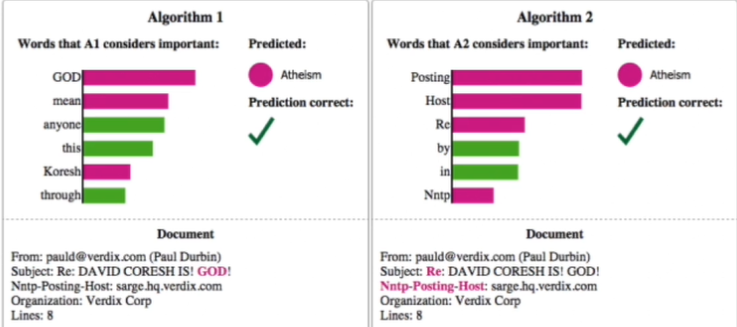
\includegraphics[width=14cm]{./capture/LIME_example.png}
  \caption{LIMEを用いて、モデルの予測根拠を解釈した図:入力にテキストデータを与え、「無神論」と「キリスト教」を分類するタスクにおいて、Algorithm 1とAlgorithm 2にLIMEを適用した結果を表している。Algorithm 2はPosting, Host, Reといった単語に着目しており、これらは無神論にもキリスト教にも関係のない単語であることから、学習データに問題があったということが分かった。}
  \label{fig:LIME_example}
\end{figure}
LIMEの実装は、https://github.com/marcotcr/lime を参考にすると良い。

\clearpage
\section{SHAP}
SHAP(Shapley Additive Explanations)は、ゲーム理論に基づいたモデル解釈手法であり、モデルの予測根拠を解釈するための手法である。SHAPは、特徴量の重要度を評価するために、Shapley値を用いる。Shapley値は、特徴量の重要度を評価するための指標であり、特徴量の組み合わせに対する貢献度を評価することができる。
\par
SHAPの概念を、A, B, Cの三人で得られる報酬額を計算する例で説明する。A, B, Cの三人が得られる報酬額を計算する際、A, B, C一人ひとりが得られる報酬額を計算する(図\ref{fig:SHAP_ABC_price})。次に、A, B, Cの二人組が得られる報酬額を計算する。この6通りの情報を元に、「限界貢献度」を計算する。例えば、Aが得られる報酬額を計算する際、A, B, Cの三人で得られる報酬額から、A以外の二人で得られる報酬額を引いたものがAの限界貢献度となる。その後、BとCの二人で得られる報酬額から、B一人の報酬額を引いたものが、Cの限界貢献度となる。さらに、Bの限界貢献度は、B一人での報酬額となる (順序によって異なる結果となる)。これらの限界貢献度をすべての通りで計算したものが、図\ref{fig:SHAP_ABC_dedication}である。こうして求まった限界貢献度の算術平均が、shapley値となる。

\begin{figure}[htbp]
  \centering
  \begin{subfigure}[b]{0.45\textwidth}
    \centering
    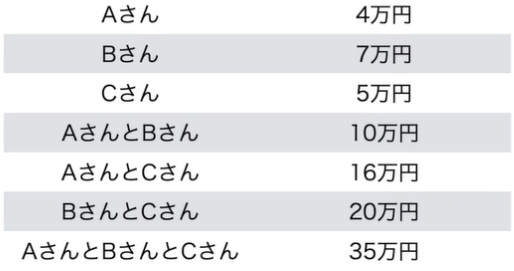
\includegraphics[width=\textwidth]{./capture/SHAP_ABC_price.png}
    \caption{A, B, Cの三人で得られる報酬額}
    \label{fig:SHAP_ABC_price}
  \end{subfigure}
  \hfill
  \begin{subfigure}[b]{0.45\textwidth}
    \centering
    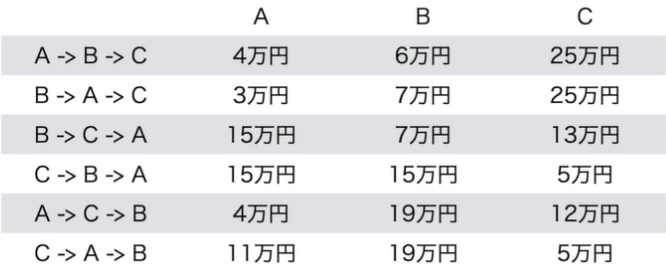
\includegraphics[width=\textwidth]{./capture/SHAP_ABC_dedication.png}
    \caption{限界貢献度のマトリクス:平均的な限界貢献度は、A=8.7, B=12.2, C=14.2となる。(算術平均)}
    \label{fig:SHAP_ABC_dedication}
  \end{subfigure}
  \caption{SHAPの概念}
\end{figure}
\par
SHAPを機械学習に適用するときは、特徴量が上述の例のA, B, Cに対応する。SHAPは、特徴量の組み合わせに対する貢献度を評価することができるため、特徴量の重要度を評価することができる。SHAPの特徴は、特徴量の重要度を評価するだけでなく、特徴量の組み合わせに対する貢献度を評価することができる点である。
\par
SHAPを用いて、Bostonデータセットを解釈した結果を図\ref{fig:SHAP_example}に示す。
\begin{figure}
  \centering
  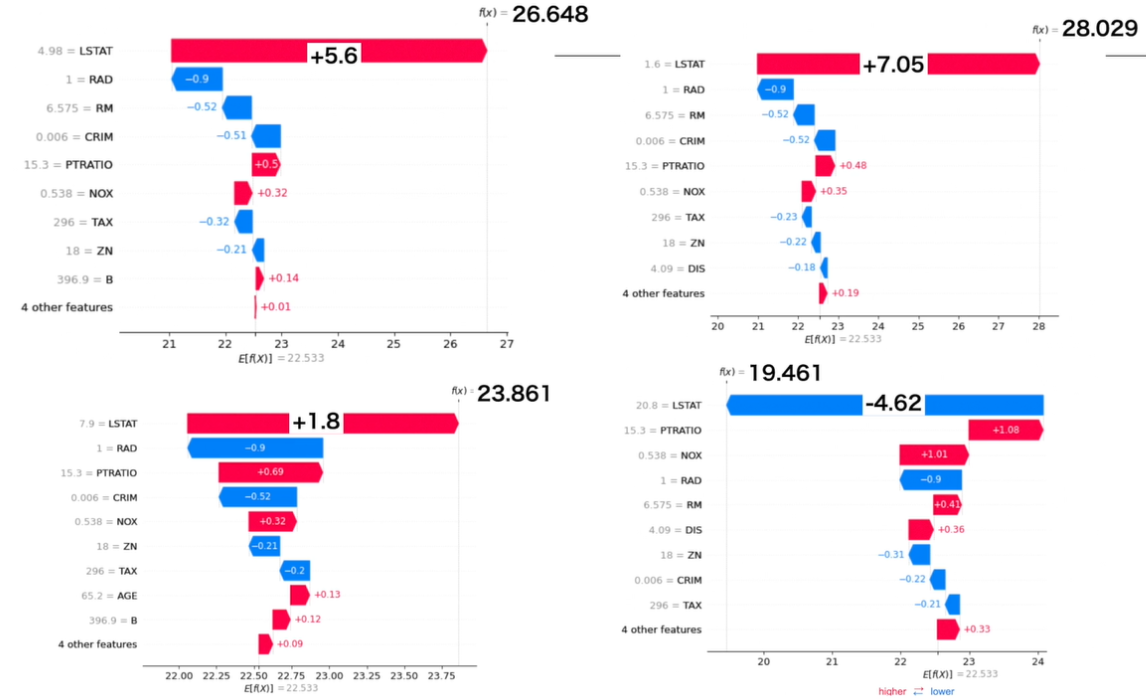
\includegraphics[width=14cm]{./capture/SHAP_Boston_dataset.png}
  \caption{Bostonデータセットを用いて、SHAPを適用した結果:左上はLSTAT(低所得者率)=4.98の場合、右上 LSTAT=1.6, 左下 LSTAT=7.9, 右下 LSTAT=20.8の場合のshapley値(限界貢献度)$f(x)$を示している。LSTATが低いほど、住宅価格を高く予測するのに働き、LSTATが高いほど、住宅価格を低く予測するのに働いていることが読み取れる。}
  \label{fig:SHAP_example}
\end{figure}

\clearpage
\paragraph{参考文献}
\begin{enumerate}
  \item 岡谷貴之/深層学習 改訂第2版 [機械学習プロフェッショナルシリーズ]/ 講談社サイエンティフィク/ 2022-01-17
  \item LIMEで機械学習の予測結果を解釈してみる \url{https://qiita.com/fufufukakaka/items/d0081cd38251d22ffebf}
  \item 機械学習モデルの局所的な解釈(LIMEとSHAP) \url{https://horomary.hatenablog.com/entry/2019/09/16/000110}
\end{enumerate}

\clearpage
\section{実装演習キャプチャ}
%------------
% Interpretability
%------------
\subsection{CAM}
\begin{figure}[htbp]
  \centering
  \includegraphics[width=10cm]{C:/Users/hiroh/Videos/Captures/4_8_interpretablitity/Arc 2024_07_15 21_14_10.png}
\end{figure}
\begin{figure}[htbp]
  \centering
  \includegraphics[width=10cm]{C:/Users/hiroh/Videos/Captures/4_8_interpretablitity/Arc 2024_07_15 21_14_30.png}
\end{figure}
\begin{figure}[htbp]
  \centering
  \includegraphics[width=10cm]{C:/Users/hiroh/Videos/Captures/4_8_interpretablitity/Arc 2024_07_15 21_14_54.png}
\end{figure}
\begin{figure}[htbp]
  \centering
  \includegraphics[width=10cm]{C:/Users/hiroh/Videos/Captures/4_8_interpretablitity/Arc 2024_07_15 21_15_04.png}
\end{figure}

\newpage
\end{document}